%----------------------------------------------------------------
%
%  File    :  survey-intro.tex
%
%  Author  :  Keith Andrews, IICM, TU Graz, Austria
% 
%  Created :  27 May 1993
% 
%  Changed :  16 Nov 2010
% 
%----------------------------------------------------------------


\chapter{Screen Readers}

\label{chap:Intro}



Screen readers are software applications, primarily used by visually impaired people. Screen readers convert web content (text, buttons, images, and other elements) into speech or braille output. Screen readers attempt to convey what visually non-impaired people see on a display via non-visual means like text-to-speech, sound icons, or a braille device.

In May - June 2021, WebAIM surveyed the  preferences of screen reader users. They received 1568 valid responses. Figure~\ref{fig:screen-readers-piechart} shows the primary screen readers preferences. The majority of users use JAWS and NVDA screen readers as their primary screen readesr. Figure~\ref{fig:screen-readers-line} shows historical trends for primary screen reader usage. After a decade of decreases in primary usage, JAWS is once again the most used screen reader, with NVDA and VoiceOver both decreasing in primary usage over the last two years.

In this paper, we focus on JAWS, NVDA, VoiceOver, Narrator, and TalkBack screen readers. They are further described in the sections below.

\begin{figure}[tp]
\centering
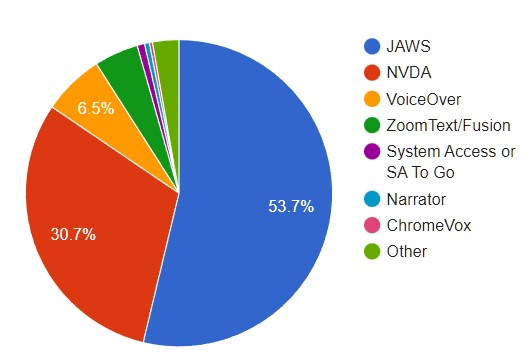
\includegraphics[keepaspectratio,width=\linewidth,height=\halfh]
{images/screen-readers-piechart.jpg}

\caption[Primary screen reader]{
Primary screen reader.
\imgcredit{Image extracted from WebAIM. ©2022 WebAIM.}
}
\label{fig:screen-readers-piechart}
\end{figure}

\begin{figure}[tp]
\centering
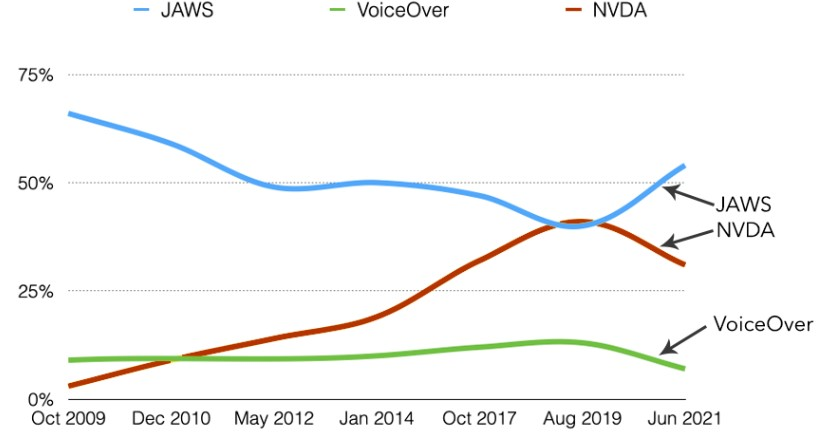
\includegraphics[keepaspectratio,width=\linewidth,height=\halfh]
{images/screen-readers-line.jpg}

\caption[Historical trends for primary screen reader]{
Historical trends for the primary screen reader.
\imgcredit{Image extracted from WebAIM. ©2022 WebAIM.}
}
\label{fig:screen-readers-line}
\end{figure}




\section{JAWS}
JAWS is the most popular screen reader for Windows computers, however, it has a learning curve. JAWS has the most configurable options among the reviewed screen readers. JAWS is only available as paid software, either as an enterprise or single-use package (90 EUR a year or approximately 900 EUR as a one-time purchase). JAWS demands a lot of the computer's RAM and can occasionally slow the computer down. JAWS supports 10 languages.

\section{NVDA}

NVDA is the second most popular screen reader for Windows computers. NVDA is available as free and open-source software. NVDA supports web content using JavaScript and supports Mozilla Firefox, Microsoft Internet Explorer, Word, Excel, Outlook, and Mozilla Thunderbird. NVDA supports 63 languages.

\section{VoiceOver}

VoiceOver is free and comes included with all Apple products. VoiceOver requires no installation or setup.VoiceOver is user-friendly and configurable. The learning curve takes some effort. VoiceOver supports 64 languages.

\section{Narrator}

Narrator is free and comes included with the Windows operating system. Narrator requires no installation or setup. Narrator offers limited functionality with web  browsers and web apps, especially with navigation and deeper levels of the Windows operating system. Narrator supports 49 languages.

\section{TalkBack}

TalkBack is free and open-source. TalkBack comes included with the Android operating system. TalkBack requires no installation or setup. TalkBack is user-friendly, however, the learning curve takes some effort. TalkBack supports 63 languages.

\section{Screen Readers Conclussion}

A comparison of information can be seen in  Table~\ref{tab:screen-readers-info}. All screen readers in question, except Narrator, are maintained regularly. JAWS, NVDA, and Narrator are available on Windows, VoiceOver is available on iOS and macOS, and TalkBack is available on Android. JAWS supports 10 languages while other screen readers support between 49 and 64 languages. JAWS is the only screen reader available as paid software while other screen readers are available as free software (NVDA and TalkBack are also open-source).

\begin{table}[tp]
\tablestretch
\rowcolors{2}{}{tablerowcolour}
\centering
\begin{tabularx}{\linewidth}
{>{\kern-\tabcolsep}lllXX<{\kern-\tabcolsep}}
\toprule
\textbf{Screen reader} & \textbf{Last update} & \textbf{System} & \textbf{Licence} & \textbf{No. of lang.} \\
\midrule
JAWS & 25. 10. 2022 & Windows & Commercial & 10 \\
%
NVDA & 1. 3. 2022 & Windows & Free and open-source & 63 \\
%
VoiceOver & 24. 10. 2022 & iOS, macOS & Free & 64 \\
%
Narrator & 2020 & Windows & Free & 49 \\
%
TalkBack & 27. 10. 2022 & Android & Free and open-source & 63 \\
\bottomrule
\end{tabularx}

\caption[Screen Readers Information]
{
Screen readers information
}
\label{tab:screen-readers-info}
\end{table}


